% Aktivierungsübersicht, ergänzt am 29.09.2026.
\question{Aktivierungsfunktionen: Formel, Kurve und Einsatz}
Nach der gewichteten Summe wird die Aktivierungsfunktion angewendet:
\[\mathbf z=\mathbf W\mathbf a+\mathbf b,\qquad \mathbf a_{\mathrm{neu}}=f(\mathbf z).\]
Ohne nichtlineare Aktivierungen ließen sich mehrere affine Schichten zu einer einzigen affinen Abbildung zusammenfassen. Aktivierungen ermöglichen komplexere Zusammenhänge.

\textbf{Kurven lesen:} Waagerecht steht der Eingang $z$, senkrecht die Ausgabe $f(z)$. Die senkrechten Achsen haben unterschiedliche Skalen.

\begingroup\small\setlength{\tabcolsep}{5pt}\renewcommand{\arraystretch}{1.12}
\begin{tabular}{@{}p{0.43\linewidth}p{0.52\linewidth}@{}}\toprule\textbf{Funktion, Kurve und Formel} & \textbf{Wann und warum?}\\\midrule
\begin{minipage}[t]{\linewidth}\vspace{0pt}\textbf{ReLU}\par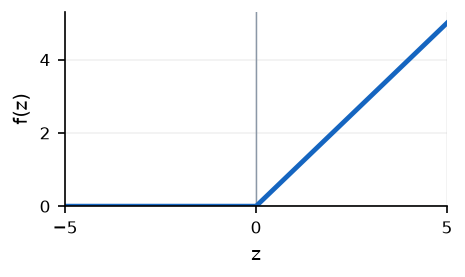
\includegraphics[width=0.85\linewidth]{figures/aktivierungsfunktionen/relu.png}\par $f(z)=\max(0,z)$\\[3pt]Bereich: $[0,\infty)$\end{minipage} & \begin{minipage}[t]{\linewidth}\vspace{0pt}\textbf{Versteckte MLP-Schichten.} Negative Werte werden null, positive bleiben unverändert. Einfach zu berechnen; für $z>0$ ist die Ableitung eins.\\[3pt]\textbf{Grenze:} Ein Neuron kann dauerhaft im negativen, inaktiven Bereich bleiben.\end{minipage}\\[7pt]\midrule
\begin{minipage}[t]{\linewidth}\vspace{0pt}\textbf{Sigmoid}\par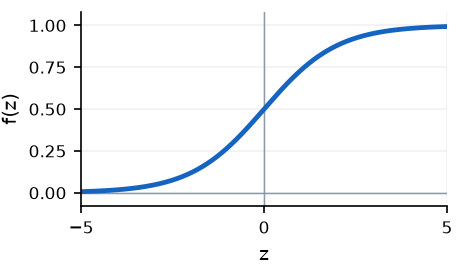
\includegraphics[width=0.85\linewidth]{figures/aktivierungsfunktionen/sigmoid.png}\par $\displaystyle\sigma(z)=\frac{1}{1+e^{-z}}$\\[3pt]Bereich: $(0,1)$\end{minipage} & \begin{minipage}[t]{\linewidth}\vspace{0pt}\textbf{Gates in LSTM/GRU:} steuert den durchgelassenen Informationsanteil. \textbf{SOC-Ausgang:} begrenzt auf null bis eins.\\[3pt]\textbf{Grenze:} Für große positive oder negative Eingaben wird die Kurve flach; der Gradient wird klein.\end{minipage}\\[7pt]\midrule
\begin{minipage}[t]{\linewidth}\vspace{0pt}\textbf{tanh}\par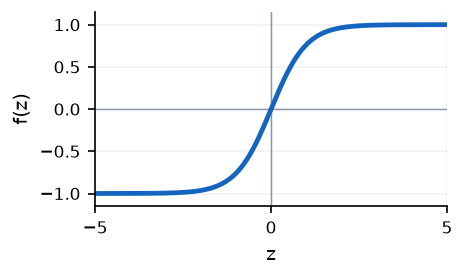
\includegraphics[width=0.85\linewidth]{figures/aktivierungsfunktionen/tanh.png}\par $\displaystyle f(z)=\frac{e^z-e^{-z}}{e^z+e^{-z}}$\\[3pt]Bereich: $(-1,1)$\end{minipage} & \begin{minipage}[t]{\linewidth}\vspace{0pt}\textbf{Zustandskandidaten in LSTM/GRU.} Erlaubt positive und negative Informationen bei begrenzter Größe. Beim LSTM auch zur Bildung von $h_t$ aus $c_t$.\\[3pt]\textbf{Grenze:} ebenfalls kleine Gradienten in den flachen Randbereichen.\end{minipage}\\[7pt]\midrule
\end{tabular}\endgroup

\clearpage
\question{Weitere Aktivierungen und die Zuordnung zu euren Modellen}
\begingroup\small\setlength{\tabcolsep}{5pt}\renewcommand{\arraystretch}{1.12}
\begin{tabular}{@{}p{0.43\linewidth}p{0.52\linewidth}@{}}\toprule\textbf{Funktion, Kurve und Formel} & \textbf{Wann und warum?}\\\midrule
\begin{minipage}[t]{\linewidth}\vspace{0pt}\textbf{GELU}\par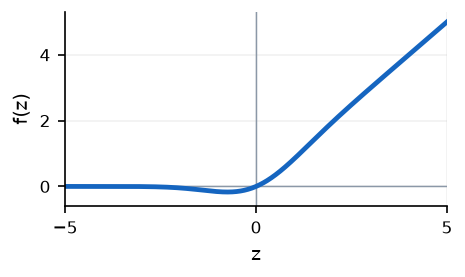
\includegraphics[width=0.85\linewidth]{figures/aktivierungsfunktionen/gelu.png}\par $f(z)=z\,\Phi(z)$\\[3pt]$\Phi$: Verteilungsfunktion der Standardnormalverteilung.\\Bereich: ungefähr $[-0{,}170,\infty)$\end{minipage} & \begin{minipage}[t]{\linewidth}\vspace{0pt}\textbf{Versteckte Schichten.} Glatter Übergang statt des ReLU-Knicks; negative Werte werden weich abgeschwächt. Im umfangreicheren SOH-Modell verwendet.\\[3pt]\textbf{Grenze:} aufwendiger als ReLU; ein Genauigkeitsvorteil ist hier nicht isoliert nachgewiesen.\end{minipage}\\[7pt]\midrule
\begin{minipage}[t]{\linewidth}\vspace{0pt}\textbf{Identität}\par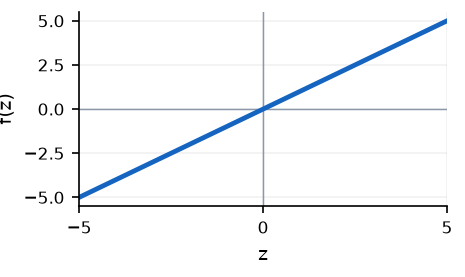
\includegraphics[width=0.85\linewidth]{figures/aktivierungsfunktionen/linear.png}\par $f(z)=z$\\[3pt]Bereich: alle reellen Zahlen.\end{minipage} & \begin{minipage}[t]{\linewidth}\vspace{0pt}\textbf{Linearer Regressionsausgang.} Lässt die berechnete Ausgabe unverändert, etwa beim eingebetteten SOH-Modell.\\[3pt]\textbf{Grenze:} keine automatische Begrenzung auf physikalisch sinnvolle Werte.\end{minipage}\\[7pt]\midrule
\end{tabular}\endgroup

\question{Welche Funktionen werden tatsächlich eingesetzt?}
\begingroup\small\setlength{\tabcolsep}{4pt}
\begin{tabular}{@{}p{0.40\linewidth}p{0.21\linewidth}p{0.15\linewidth}p{0.15\linewidth}@{}}
\toprule Modell & Rekurrenter Teil & Versteckte MLP-Schichten & Ausgang\\\midrule
SOC-GRU, Kapitel 6 & Sigmoid, tanh & ReLU & Sigmoid\\[5pt]
Umfangreicheres SOH-LSTM, Kapitel 6 & Sigmoid, tanh & GELU & Linear\\[5pt]
Eingebettetes SOC-LSTM, Kapitel 7 & Sigmoid, tanh & ReLU & Sigmoid\\[5pt]
Eingebettetes SOH-LSTM, Kapitel 7 & Sigmoid, tanh & ReLU & Linear\\\bottomrule
\end{tabular}\endgroup

GELU wird im umfangreicheren SOH-Modell auch in der Eingangsverarbeitung und den Residualblöcken verwendet. Gemeint ist jeweils der Netzausgang vor einer möglichen nachgeschalteten Filterung oder Begrenzung.

\textbf{LSTM-Merker:} Der Cell State selbst wird nicht einfach durch tanh begrenzt. Für den Hidden State gilt $h_t=o_t\odot\tanh(c_t)$.

\textbf{Codebasis:} Überprüft wurden die GRUMLP-Definition im SOC/SOH-Simulationsskript, das SOH-Modell 0.1.2.3 in predict\_soh.py sowie die SOC- und SOH-LSTM-Basisimplementierungen der STM32-Firmware. Stand: 29.09.2026.
\clearpage
\question{Ergänzende Vergleichsfunktionen: Leaky ReLU und Softmax}
Diese beiden Funktionen dienen der Einordnung. Sie sind nicht die Aktivierungen der auf der vorigen Seite aufgeführten Modellimplementierungen.

\begingroup\small\setlength{\tabcolsep}{5pt}\renewcommand{\arraystretch}{1.12}
\begin{tabular}{@{}p{0.43\linewidth}p{0.52\linewidth}@{}}\toprule\textbf{Funktion, Kurve und Formel} & \textbf{Wann und warum?}\\\midrule
\begin{minipage}[t]{\linewidth}\vspace{0pt}\textbf{Leaky ReLU}\par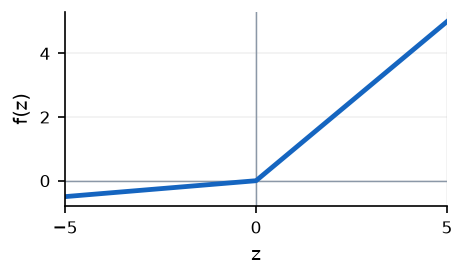
\includegraphics[width=0.85\linewidth]{figures/aktivierungsfunktionen/leaky_relu.png}\par $f(z)=\max(\alpha z,z)$\\[3pt]$0<\alpha<1$; hier $\alpha=0{,}1$.\\Bereich: alle reellen Zahlen.\end{minipage} & \begin{minipage}[t]{\linewidth}\vspace{0pt}\textbf{Alternative für versteckte Schichten.} Negative Eingaben behalten einen kleinen Gradienten. Das schwächt das Problem dauerhaft inaktiver ReLU-Neuronen ab.\\[3pt]In den zuvor zugeordneten Modellimplementierungen nicht verwendet.\end{minipage}\\[7pt]\midrule
\begin{minipage}[t]{\linewidth}\vspace{0pt}\textbf{Softmax}\par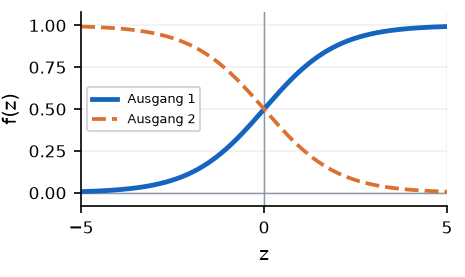
\includegraphics[width=0.85\linewidth]{figures/aktivierungsfunktionen/softmax.png}\par $\displaystyle f_i(\mathbf z)=\frac{e^{z_i}}{\sum_j e^{z_j}}$\\[3pt]Bei mindestens zwei Ausgängen: jeder in $(0,1)$; Summe eins.\end{minipage} & \begin{minipage}[t]{\linewidth}\vspace{0pt}\textbf{Klassifikation mit sich ausschließenden Klassen.} Verarbeitet mehrere Werte gemeinsam. Grafik: $\mathbf z=(z,0)$; blau erster, orange zweiter Ausgang.\\[3pt]\textbf{Kein einzelner SOC-Ausgang:} Bei nur einem Ausgang wäre Softmax immer eins.\end{minipage}\\[7pt]\midrule
\end{tabular}\endgroup

\question{Was sollte ich für die Verteidigung mitnehmen?}
ReLU und GELU verarbeiten Merkmale in versteckten Schichten. Sigmoid steuert Gates oder begrenzt Ausgaben. Tanh ermöglicht begrenzte Werte mit beiden Vorzeichen. Ein linearer Ausgang lässt die letzte berechnete Größe unverändert.

\textbf{Begriffe trennen:} Eine Linear-Schicht berechnet die affine Abbildung $Wa+b$. Eine anschließende Identitätsaktivierung verändert dieses Ergebnis nicht. Softmax ist dagegen eine gemeinsame Operation über mehrere Ausgänge.
\clearpage
